\chapter{Základné pojmy}
\label{kap:kapitola1} % id kapitoly pre pre prikaz ref

\section{Jednoparametrický systém}
Ak nakreslíme kružnice so stredom na x-ovej osi s polomerom 1, ako na obrázku, pohľad nám upútajú horizontálne priamky $y = \pm 1$ idúce ponad a popod systém kružníc.

\begin{figure}[h]
	\centering
	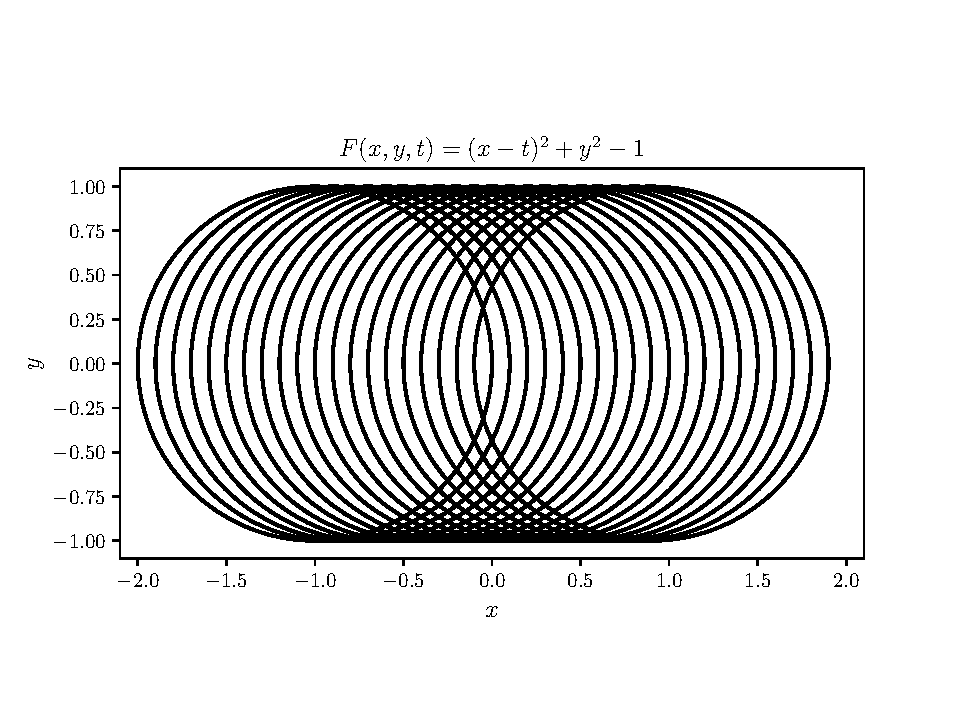
\includegraphics{images/system.pdf}
	\caption[Systém kružníc.]{Systém kružníc.}
	\label{fig:system}
\end{figure}

Každá z týchto priamok sa dotýka každej kružnice v jednom bode a v tomto bode majú spoločnú dotyčnicu. V nasledovnom texte túto myšlienku matematicky opíšeme, na základe nej zostrojíme tzv. obálku systému kriviek alebo plôch a porovnáme prístupy ich výpočtu. Budeme pracovať v reálnom vektorovom priestore so štandardným skalárnym súčinom, teda v euklidovskom priestore, rozmeru $n = 2, 3.$ Najprv ilustrujeme príklady obálok a ich výpočet pre $ n = 2.$ Po celý čas predpokladáme, že všetky zobrazenia sú dostatočne veľakrát diferencovateľné. Tučným písmom značíme vektorovú funkciu a parametre pre prehľadnosť zápisov vynechávame, ak sú z kontextu zrejmé.

Vo všeobecnosti, začneme v $\mathbb{R}^2$ s jednoparametrickým systémom kriviek daným funkciou, v $\mathbb{R}^3$ máme jednoparametrický systém plôch.

\begin{definition}
Nech $F \colon \mathbb{R}^{n} \times I \rightarrow \mathbb{R}$ je funkcia v premenných $ x_{1}, x_{2}, \ldots, x_{n} $ a v parametri $t$, kde $I \subseteq \mathbb{R}$ je interval. Definujeme jednoparametrický systém nadplôch ako systém množín 
$$
\mathcal{F}_{t} = \{ (x_{1}, x_{2}, \ldots, x_{n}) \in \mathbb{R}^{n}, \ F(x_{1}, x_{2}, \ldots, x_{n}, t) = 0, \ t \in I \}.
$$
\end{definition}

V $n = 2$ budeme pre lepšiu prehľadnosť značiť premenné $x_{1}, x_{2}$ ako $x, y,$ pre $n = 3$ pribudne $x_{3}$ ako $z.$

Pre horeuvedený prípad teda máme jednoparameterický systém kružníc so stredmi kružníc, ktoré ležia na úsečke parametrizovanej $(t,0)$ pre $t \in [-1,1]$ a konštantným polomerom pre každú kružnicu $r = 1$ daný implicitnou funkciou
$$ \mathcal{F}_{t} = \{ (x, y) \in \mathbb{R}^{2} \mid \ F(x, y, t) = 0, \ t \in [-1,1] \}, $$
kde
$$ F(x, y, t) = (x - t)^2 + y^2 - 1.$$

Systém budeme ilustrovať zobrazením niektorých prvkov systému pre diskrétne hodnoty parametra $t$. Pre $t = -1$ je zodpovedajúca $F_{-1} \in \mathcal{F}_{t}$  kružnica s implicitnou rovnicou
$$ F_{-1}(x, y) = F(x, y, -1) = (x + 1)^2 + y^2 - 1. $$

\begin{figure}[H]
	\centering
	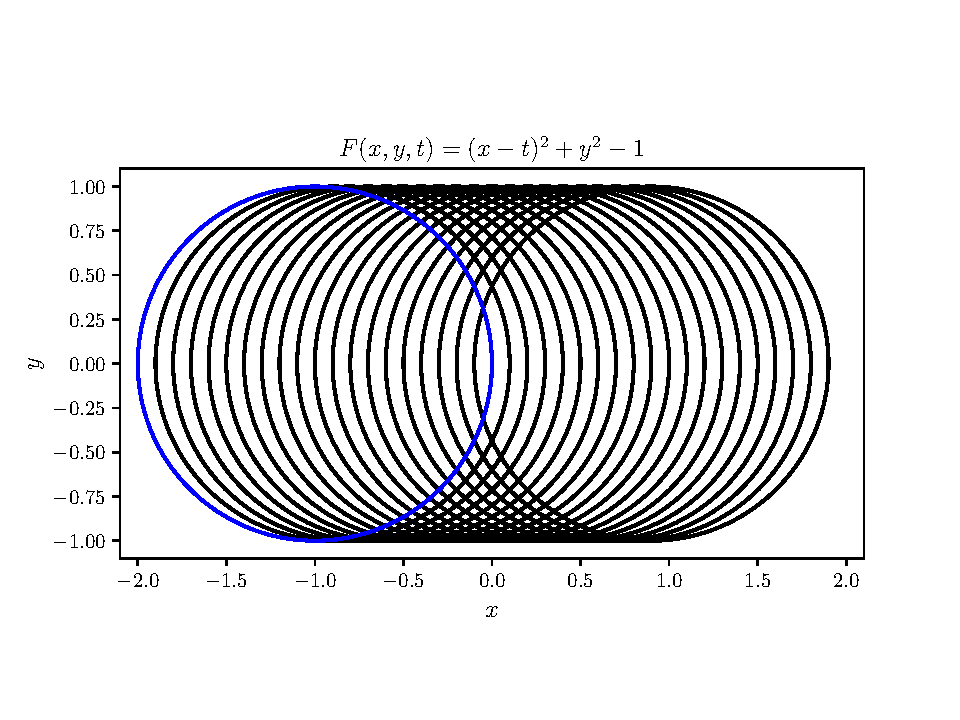
\includegraphics{images/one_element_of_system.pdf}
	\caption[Zobrazenie prvkov systému.]{Modrou farbou je vyznačená kružnica systému v parametri $t=-1$.}
	\label{fig:one_element_of_system}
\end{figure}

\section{Obálka jednoparametrického systému nadplôch}
Najskôr definujeme obálku jednoparametrického systému kriviek v $\mathbb{R}^2$. Uvedieme charakterizáciu obálok, ktorú možno použiť na výpočet pre jednoduchšie jednoparametrické systémy. Následne túto charakterizáciu použijeme ako definíciu pre obálku jednoparametrického systému plôch v $\mathbb{R}^n$.

Definujme gradient $\nabla F(x,y,t) $ vzhľadom na $x$ a $y$ ako
$$\nabla F(x, y, t) = \left(\frac{\partial F}{\partial x}(x, y, t), \frac{\partial F}{\partial y}(x, y, t) \right).$$ Predpokladáme, že $\nabla F(x,y,t) \neq \vec{0}. $ 

\begin{definition}
Obálkou systému kriviek $ \mathcal{F}_{t} $ je parametrizovaná krivka $\gamma(t) \colon J \subseteq I \rightarrow \mathbb{R}^{2}$ taká, že 
\begin{enumerate}
\item $\gamma(t) \in \mathcal{F}_{t} \text{ pre všetky } t \in J,$
\item $\dot{\gamma}(t) \perp \nabla F \left( \gamma(t), t \right).$
\end{enumerate}
\end{definition}

Obálka $\gamma(t)$ sa dotýka každej krivky zo systému $F(x,y,t)$ v bode $(x, y)$  pre nejaké $t$ a v tomto bode má s krivkou zo systému rovnakú dotyčnicu. To znamená, že každý bod obálky ${\gamma}(t) = (\gamma_{1}(t),\gamma_{2}(t))$ spĺňa rovnicu systému $F(\gamma_{1}(t),\gamma_{2}(t),t)=0$ pre nejaké $t,$ a teda platí prvá podmienka $\gamma(t) \in \mathcal{F}_{t}$. Gradient funkcie $ \nabla F(x,y,t)$ je normálový vektor k $F(x,y,t)$ v regulárnom bode $(x,y)$ a parametri $t$. V spoločnom bode $(x,y)$ a parametri $t$ chceme rovnaký smer dotykového vektora pre $\gamma(t)$ a $F(x,y,t), $ z čoho vyplýva, že $\dot{\gamma}(t)$ a dotykový vektor k funkcii $F(x,y,t)$ sú lineárne závislé, z čoho dostávame $\dot{\gamma}(t) \perp \nabla F \left( \gamma(t), t \right), $ druhú podmienku v definícii obálky. Interval $J,$ na ktorom dostávame výslednú obálku môže byť menší ako interval $I,$ na ktorom bol definovaný systém kriviek, teda máme $J \subseteq I.$ Ak by bol gradient $\nabla F(x,y,t) $ v nejakom bode nulový, nevieme nájsť jednoznačne dotykový vektor obálky a systému. 

\begin{theorem}
Regulárna krivka $\gamma(t) \colon J \subseteq I \rightarrow \mathbb{R}^{2}$ kde $t \in J  \subseteq I$ je obálkou jednoparametrického systému $\mathcal{F}_{t}$ práve vtedy, keď spĺňa:
\begin{enumerate}
\item $F(\gamma(t), t) = 0, $ 
\item $\dfrac{\partial F}{\partial t}(\gamma(t), t) = 0.$
\end{enumerate}
\end{theorem}

\begin{proof}
Táto odlišná charakterizácia je ekvivalentná definícii, ktorú sme postavili na geometrických podmienkach. Stačí zistiť korešpondenciu podmienok.
\begin{enumerate}
\item Ako sme už vysvetlili, každý bod obálky ${\gamma}(t) = (\gamma_{1}(t),\gamma_{2}(t))$ spĺňa rovnicu jednoparametrického systému $F(\gamma_{1}(t),\gamma_{2}(t),t)=0$ pre nejaké $t,$ teda podmienky 
$$ F(\gamma(t), t) = F(\gamma_{1}(t), \gamma_{2}(t), t) = 0$$
a
$$\gamma(t) \in \mathcal{F}_{t}$$
sú ekvivalentné.
\item Derivujme $F(\gamma_{1}(t),\gamma_{2}(t), t)$ podľa parametra $t,$ kde $ \dot{\gamma}(t) = ( \dot{\gamma_{1}}(t), \dot{\gamma_{2}}(t) ).$
$$ \frac{\partial F}{\partial x}(\gamma_{1}(t),\gamma_{2}(t),t) \cdot \dot{\gamma_{1}}(t)+\frac{\partial F}{\partial y}(\gamma_{1}(t),\gamma_{2}(t),t) \cdot \dot{\gamma_{2}}(t)+\frac{\partial F}{\partial t}(\gamma_{1}(t),\gamma_{2}(t),t) \cdot 1 = 0. $$
Nakoľko požadujeme, aby gradient funkcie $\nabla F(\gamma_{1}(t),\gamma_{2}(t),t)$ bol kolmý na $\dot{\gamma}(t) \text{ tak}$
$$ \langle \nabla F(\gamma_{1}(t),\gamma_{2}(t),t), \dot{\gamma}(t) \rangle = 0,$$
teda platí
$$ \frac{\partial F}{\partial x}(\gamma_{1}(t),\gamma_{2}(t),t) \cdot \dot{\gamma_{1}}(t)+\frac{\partial F}{\partial y}(\gamma_{1}(t),\gamma_{2}(t),t) \cdot \dot{\gamma_{2}}(t) = 0, $$
z čoho dostávame
$$ \frac{\partial F}{\partial t}(\gamma_{1}(t),\gamma_{2}(t),t) = 0. $$ 
\end{enumerate}
\end{proof}

Obálka sa počíta riešením rovníc
\begin{align*}
F(x, y, t) &= 0, \\
\frac{\partial F}{\partial t}(x,y,t) &= 0. \\
\end{align*}

Často sa v literatúre môžeme stretnúť s rôznymi opismi obálky, ktoré však bez ďalších predpokladov nemusia definovať rovnakú množinu bodov. Príkladom je ďalšia charakterizácia obálky ako množiny limitných bodov prienikov kriviek systému. Vzťahy medzi jednotlivými charakterizáciami možno nájsť v \cite{Bru81}.  

Dokonca, daný systém nemusí mať obálku. Príkladom sú sústredné kružnice s rastúcim polomerom.

\begin{example} 
Obálku systému sústredných kružníc pre $t \in I=[\frac{1}{10},2]$ rátame ako systém rovníc
\begin{align*}
F(x, y, t) &= x^2 + y^2 - t, \\
\frac{\partial F}{\partial t}(x,y,t) &= -1. \\
\end{align*}
Z druhej rovnice máme $t=-1 \neq 0,$ teda systém nemá riešenie. Aj keď by sa nám mohlo zdať, že by obálkou mohli byť body kružnice s najväčším polomerom $F_2$ a kružnice s najmenším polomerom $F_{\frac{1}{10}}$, práve podmienka existencie takej krivky $\gamma(t),$ ktorá by patrila do systému kružníc $\mathcal{F}_t$ pre všetky $t$ z intervalu $J \subseteq  I, $ nie je splnená.
\end{example}

\begin{figure}[H]
	\centering
	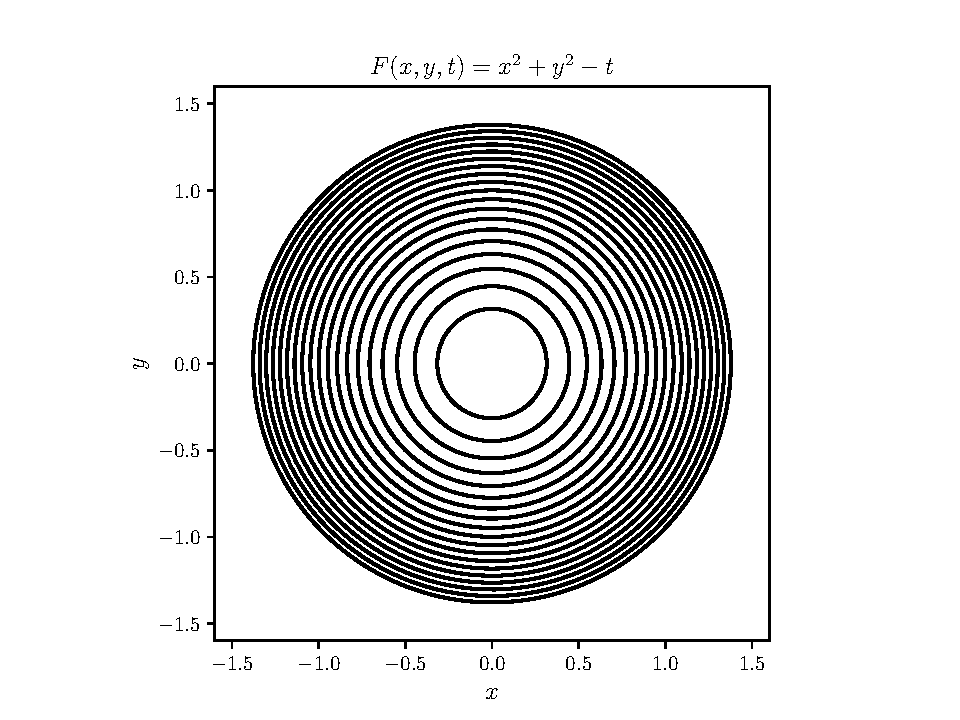
\includegraphics{images/concentric_circles.pdf}
	\caption{Sústredné kružnice.}
	\label{fig:concentric_circles}
\end{figure}


Prístup, ktorý sme využili pre jednoparametrický systém kriviek, možno zovšeobecniť pre ľubovoľný jednoparametrický systém plôch v $\mathbb{R}^n.$

\begin{definition}{\textbf{\textup{(Charakterizácia.)}}}
\label{charakterizacia}
Obálkou jednoparametrického systému plôch $ \mathcal{F}_{t} $ je množina bodov $\mathcal{E}$ daná
$$\mathcal{E} = \{(x_{1}, x_{2}, \dots, x_{n})  \in \mathbb{R}^{n} \colon \exists t \in \mathbb{R}, F(x_{1}, x_{2}, \dots, x_{n}, t) = \frac{\partial F}{\partial t}(x_{1}, x_{2}, \dots, x_{n}, t) = 0 \}.$$
\end{definition}

Ak by sme chápali obálku podľa definície ako množinu bodov, problém by sme mohli riešiť ako systém nelineárnych rovníc v parametri $t,$ kde chceme z rovníc 
\begin{align*}
F(x,y,t) &= 0, \\
\frac{\partial F}{\partial t}(x, y, t) &= 0. \\
\end{align*}
eliminovať $t.$ Na riešenie nelineárneho systému dvoch rovníc síce existujú pokročilé nástroje, no eliminovaním parametra $t$ strácame informáciu o tom, kde je obálka definovaná. 

\begin{example}
Pre náš príklad $ F(x, y, t) = (x - t)^2 + y^2 - 1 = 0 $ máme 
$$\frac{\partial F}{\partial t}(x, y, t) = 2(t-x) = 0. $$
Ak $t = x, $ tak $y^2 = 1.$ Teda obálka je podľa tejto charakterizácie $ y = \pm 1, $ ako sme očakávali.
\end{example}

\begin{figure}[H]
	\centering
	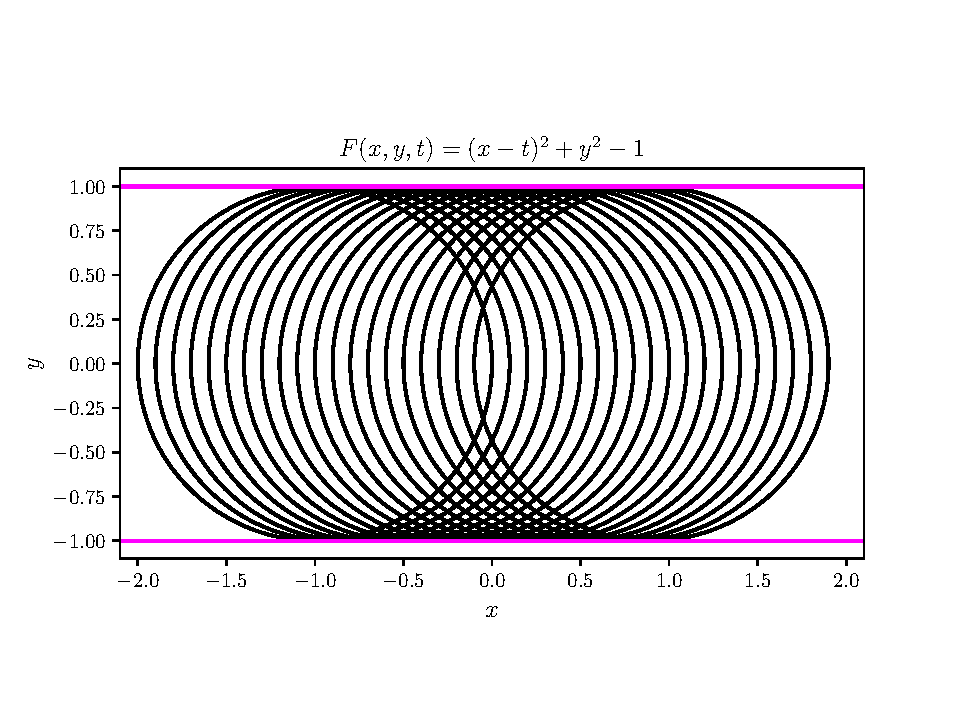
\includegraphics{images/system_with_envelope_unlimited_domain.pdf}
	\caption{Obálka systému podľa charakterizácie.}
	\label{fig:system_with_envelope_unlimited_domain}
\end{figure}

V skutočnosti sú obálkou úsečky $y=\pm 1$ definované na intervale $[-1,1]$.

\begin{figure}[H]
	\centering
	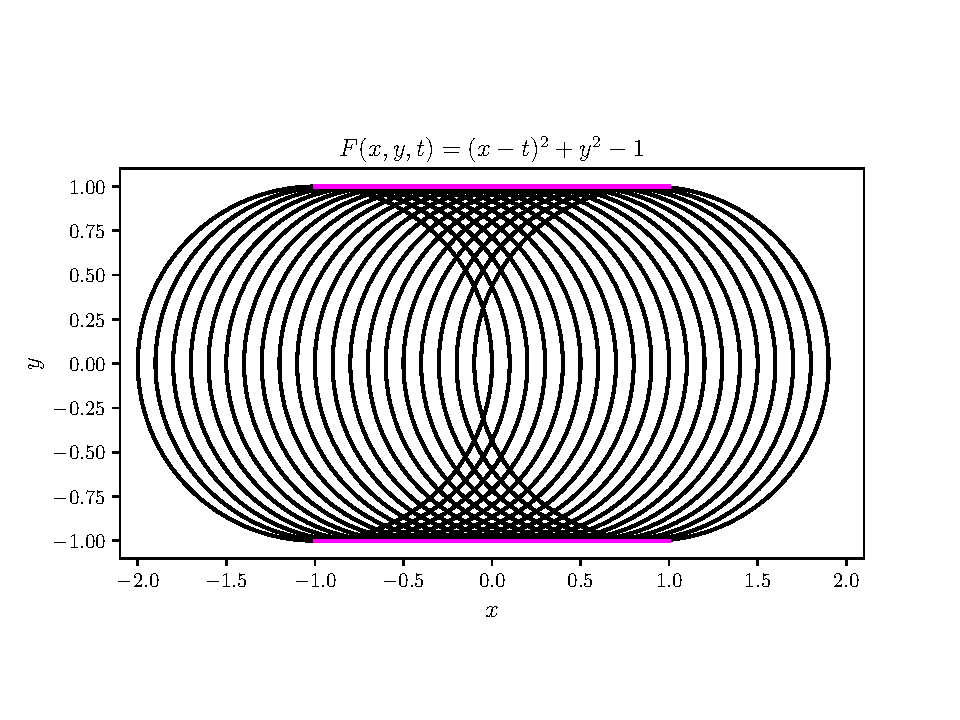
\includegraphics{images/system_with_correct_envelope.pdf}
	\caption{Obálka systému podľa definície.}
	\label{fig:system_with_correct_envelope}
\end{figure}

Tento problém možno ošetriť tak, že budeme uvažovať systémy kriviek, ktoré sú v parametri $t$ definované na celej reálnej priamke $\mathbb{R}$. 

\begin{example}
\label{example:too_complicated_equations}
Počítajme obálku systému kriviek, znázorneného na obrázku \ref{fig:too_complicated_equations}, ktorý je daný vzťahmi
\begin{align*}
F(x,y, t) &= \dfrac{x^2}{(t^2 + 1)^2} + (y - 2t)^2 - 1, \\
\dfrac{\partial F}{\partial t}(x, y, t) &= -\dfrac{4x^2t}{\left(t^2+1\right)^3}-4\left(y-2t\right). \\
\end{align*}
Vynásobením prvej rovnice $ \lambda(t) = (t^2 + 1)^2$ a derivovaním získavame
\begin{align*}
F^\lambda &= 4 t^6 - 4 t^5 y + t^4 y^2 + 7 t^4 - 8 t^3 y + 2 t^2 y^2 + 2 t^2 - 4 t y + x^2 + y^2 - 1, \\
F_t^\lambda &= 24t^5-20yt^4+4y^2t^3+28t^3-24yt^2+4y^2t+4t-4y. \\
\end{align*}
Na obrázku \ref{fig:too_complicated_equations} je znázornený tento systém elíps pre $t \in [-2,2]$ s krokom $\Delta t=0.1$. Obálku nájdeme ako riešenie $F^\lambda \cap F_t^\lambda. $ Rovnice sú však príliš vysokého stupňa v parametri $t$, preto nevieme implicitnú rovnicu obálky bez vhodného nástroja vyjadriť. V ďalšej časti rozoberieme prístupy výpočtu.
\end{example}

\begin{figure}[H]
	\centering
	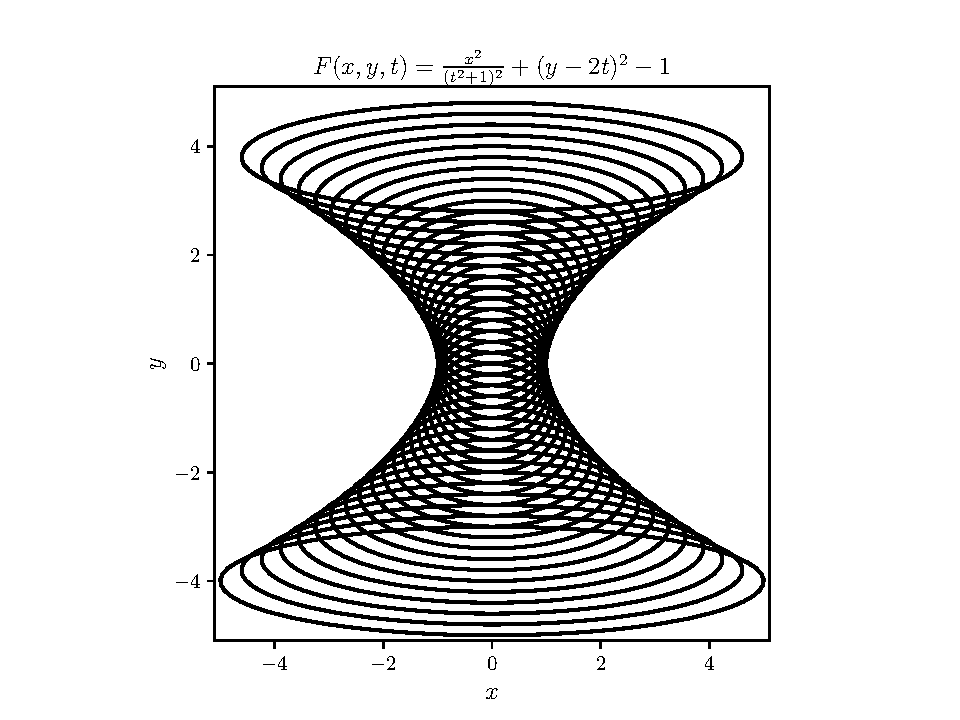
\includegraphics{images/too_complicated_equations.pdf}
	\caption{Systém elíps.}
	\label{fig:too_complicated_equations}
\end{figure}


\section{Výpočet obálky}
Vo väčšine prípadov sú rovnice charakterizujúce obálku systému plôch príliš vysokého stupňa v parametri $t$ a nedokážeme z nich ľahko odvodiť rovnicu obálky, preto pristupujeme aj k numerickým riešeniam. Spoľahlivá aproximácia obálky je jednou z aktuálnych výskumných tém. Na začiatok si však rozoberme existujúce analytické prístupy. Naledujúce prístupy sú prevzaté z \cite{Vra22}.
\subsection{Prístup algebraickej geometrie}
Dokonca aj v prípade jednoduchého príkladu ako \ref{example:too_complicated_equations}, obe polynomické rovnice charakterizujúce obálku sú vysokého stupňa v parametri $t$, preto je odstránenie parametera $t$ náročné bez vhodného nástroja. Štandardným aparátom na túto úlohu sú Gröbnerove bázy. Gröbnerove bázy sú kľúčovým pojmom v algebraickej geometrii a počítačovej algebre. Ide o špeciálnu množinu polynómov vo viacerých premenných, ktoré majú niekoľko dôležitých vlastností a zohrávajú kľúčovú úlohu pri riešení rôznych matematických problémoch vrátane riešenia sústav polynomických rovníc, zjednodušovania polynómov a dokazovania rôznych algebraických tvrdení. Vybudovanie tejto teórie je pomerne zdĺhavé, preto odkážeme na bohaté teoretické pozadie v \cite{Chalm}.
Najprv vypočítame Gröbnerovu bázu Buchbergerovým algoritmom pre ideál generovaný sústavou polynomických rovníc, ktorá obsahuje všetky premenné vrátane tej, ktorú chceme eliminovať. Z Gröbnerovej bázy vyberieme polynómy, ktoré obsahujú premennú, ktorú chceme eliminovať. Tieto polynómy použijeme na vyjadrenie tejto premennej v závislosti od ostatných premenných. Po vyriešení nových rovníc získame výraz, ktorý opisuje vzťah medzi zvyšnými premennými a eliminovanou premennou. Týmto spôsobom úspešne eliminujeme premennú.
Pokúsme sa vypočítať Gröbnerovu bázu príkladu \ref{example:too_complicated_equations} vzhľadom na lexikografické usporiadanie monómov $t > x > y $. Keďže výpočet Gröbnerovej bázy trvá pomerne dlho, neuvádzame postup a výsledok možno nájsť v prílohe \ref{pri:priloha1}.

Gröbnerova báza vzhľadom na iné usporiadanie, napr. grevlex je zvyčajne vypočítaná oveľa rýchlejšie a jej polynómy majú krajšie koeficienty, no na druhej strane, tento prístup nie je vo všeobecnosti možné použiť na odstránenie premennej $t$ z rovníc. 

Existujú aj iné metódy na riešenie polynomických rovníc, ktoré nie sú závislé na usporiadaní monómov. 
Spôsob, ako nájsť polynóm, ktorý leží v prvom eliminačnom ideáli, ktorý je nezávislý na Gröbnerovej bázach a monómických usporiadaniach, využíva teóriu rezultantov. Rezultant je determinant matice polynómov.

Hoci výpočet determinantov veľkých matíc je výpočtovo aj časovo náročný problém, existujú metódy, ako  vypočítať determinant efektívnejšie. V príklade \ref{example:too_complicated_equations} uvedieme výsledný polynóm $Res(F^\lambda , F_t^\lambda , t)$ a ukážeme obálku nájdenú rezultantom, pozri \ref{fig:resultant}. 

$ Res(F^\lambda , F_t^\lambda , t) = 191102976x^{10} + 262144x^8y^6 - 9584640x^8y^4 + 83165184x^8y^2 - 633470976x^8 - 16384x^6y^{10} - 81920x^6y^8 - 14483456x^6y^6 - 113311744x^6y^4 + 96419840x^6y^2 + 698368000x^6 - 16384x^4y^{12} - 294912x^4y^{10} - 2998272x^4y^8 - 18284544x^4y^6 - 74956800x^4y^4 - 184320000x^4y^2 - 256000000x^4. $

\begin{figure}[H]
	\centering
	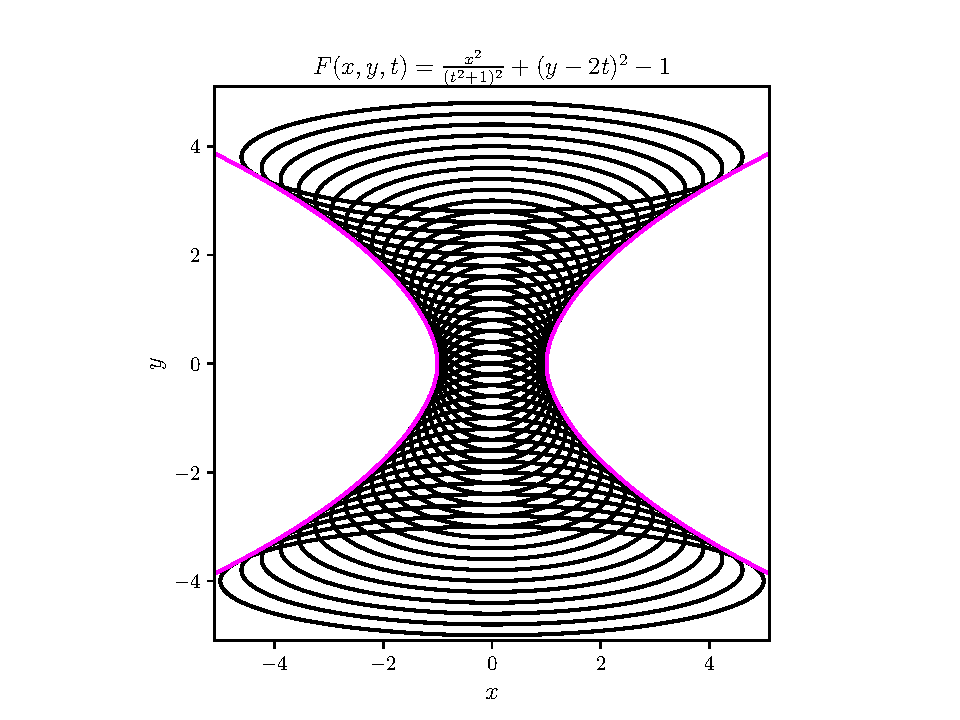
\includegraphics{images/resultant.pdf}
	\caption{Obálka vypočítaná rezultantom.}
	\label{fig:resultant}
\end{figure}

Navyše táto metóda, rovnako ako metóda založená na eliminačnej teórii s použitím Gröbnerových báz, nám vypočíta správnu obálku len vtedy, ak uvažujeme parameter $t$ jednoparametrického systému z celej reálnej priamky. Ak obmedzíme oblasť parametra na interval, tak obálka zvyčajne nemôže byť daná implicitnou rovnicou, a preto je potrebné nájsť nejakú parametrizáciu obálky. 

Pri použití rezultantov máme lepšiu kontrolu nad zložitosťou výpočtu. Pre dané dva polynómy totiž vieme, ako sa konštruuje rezultant, a tak vieme odhadnúť, s akými veľkými polynómami sa bude počas výpočtu manipulovať, avšak pri hľadaní Gröbnerovej bázy je ťažké odhadnúť, aké zložité S-polynómy sa behom algoritmu vyskytnú. Nie je zriedkavosťou, že S-polynómy sú podstatne komplikovanejšie než vstupné polynómy a výsledná Gröbnerova báza.

\subsection{Prístup projektívnej geometrie}
Body duálneho projektívneho priestoru $\mathbb{P}^3 $ možno stotožniť s nadrovinami v $\mathbb{R}^3$. Plochu v duálnom projektívnom priestore možno teda interpretovať ako množinu všetkých jej dotykových nadrovín. Pomocou duálneho prístupu sa dá dokázať, že obálky jednoparametrických systémov sú racionálne pre racionálne vstupné údaje. Potrebné teoretické pozadie možno nájsť v \cite{Pott01} a príklady pre výpočet obálky možno nájsť v \cite{Vra22}, \cite{Pet08}.
Vo všeobecnosti platí, kvadrika v $\mathbb{P}^3$ je kvadrika v duálnom projektívnom priestore, [14, Veta 1.1.35].

\begin{example}
Uvažujme systém kružníc s konštantným polomerom $\dfrac{1}{2}$, ktorých stredy ležia na rovinnej krivke $m(t) = (t^3, t^2)$, $t \in \mathbb{R}$.
$$F_{1} = \{(Q, t) \in \mathbb{R}^2 : (x - t^3)^2 + (y - t^2)^2 - \dfrac{1}{4} = 0, \ t \in \mathbb{R} \}.$$
Krivka $m_1 \subset \mathbb{R}^3$, ktorá korešponduje so systémom $F_{t}$ v cyklografickom modeli, je krivka $m_1(t) = (t^3, t^2, \dfrac{1}{2}), t \in \mathbb{R}$.
Systém 
$$F_{2} = \{(Q, t) \in \mathbb{R}^2 : (x - t^3)^2 + (y - t^2)^2 - \frac{t^2}{4} = 0, t \in \mathbb{R} \}$$
je jednoparametrický systém kružníc, kde polomery nie sú konštantné a ich stredy ležia na tej istej krivke $m(t)$ ako v predchádzajúcom prípade. Sféry korešpondujúce s $t < 0$ sú negatívne orientované a orientácia sa mení pre kruhy korešpondujúce s $t > 0$. Pre $t = 0$ je prvok $F_0 \in F_t$ bod $(0, 0) \in c(t)$, čo je guľa s nulovým polomerom a bez orientácie.
Krivka v $\mathbb{R}^3$, ktorá korešponduje s týmto systémom v cyklografickom modeli, je krivka $m_2(t) = (t^3, t^2, \dfrac{t}{2}), t \in \mathbb{R}$.
Krivka $m(t)$ je ortogonálna projekcia oboch kriviek $m_1$ a $m_2$ a často sa nazýva mediálna os jednoparametrického systému.
Pozrite si Obrázok 2.10 pre krivky $m_1, m_2 \subset \mathbb{R}^3$, jednoparametrické systémy $F_{1t}$ a $F_{2t}$ rovinných kružníc a ich mediálne osy.
$\langle \dot{m}(t), \dot{m}(t) \rangle = 9t^4 + 4t^2 + \dfrac{1}{16} \geq 0$
takisto aj 
$\langle \dot{m}(t), \dot{m}(t) \rangle = 9t^4 + 4t^2 + \dfrac{1}{4} \geq 0$
\end{example}

Rovnakým spôsobom môžeme definovať jednoparametrický systém sfér v $\mathbb{R}^3$ ako obraz kriviek v $\mathbb{R}^4$.
Jedným z dôležitých výsledkov je, že pomocou cyklografického obraz racionálnej krivky možno rozhodnúť o reálnosti obálky a to tak, že cyklografický obraz $m(t) \subset \mathbb{R}^{n+1}$ má reálnu obálku práve vtedy, keď $\langle \dot{m}(t), \dot{m}(t) \rangle \geq 0$ a rovnosť platí len pre izolované hodnoty $t$, kde $\langle \dot{m}(t), \dot{m}(t) \rangle = m_1^2(t) + m_2^2(t) + \ldots + m_n^2(t) - m_{n+1}^2(t).$

\subsection{Kinematický prístup}
Ďalším zo spôsobov, ako chápať jednoparametrické systémy plôch v $\mathbb{R}^n$ je pozerať sa na ne ako na množinu všetkých transformácií daného povrchu $P$. Povrch $P$ sa transformuje na ostatné prvky systému prostredníctvom prvkov vhodnej grupy transformácií. Táto množina transformácii má okrem štruktúry grupy aj štruktúru hladkej variety \textit{(smooth manifold)}. Tieto grupy nazývame Lieove grupy.

\begin{example}
Ilustujme tento postup na jednoduchom rovinnom príklade. Transformujme zobrazením $g_t$ priamku
\begin{align*}
l \colon x(u) &= 1 \\
y(u) &= u \\
\end{align*}
\[
g_t \begin{pmatrix} x \\ y \end{pmatrix} = \begin{pmatrix}
\cos t & -\sin t  \\
\sin t & \cos t  \\
\end{pmatrix}
\begin{pmatrix} x \\ y \end{pmatrix}.
\]
Pre každé $t \in \mathbb{R}$, $g_t$ zodpovedá rotácii. Grupa všetkých rotácií je $SO(n)$ a nazýva sa špeciálna ortogonálna grupa. Pre $t = 0$, dostávame priamku $l$. Pre iné $t$, napríklad $t = \frac{\pi}{2}$, dostávame priamku
\begin{align*}
g_t(l) \colon x(u) &= -u \\
y(u) &= 1. \\
\end{align*}
Na obrázku \ref{fig:lines_in_normal_form} je znázornená priamka $l$ modrou farbou, transformovaná priamka $g_t(l)$ červenou farbou.

\begin{figure}[H]
	\centering
	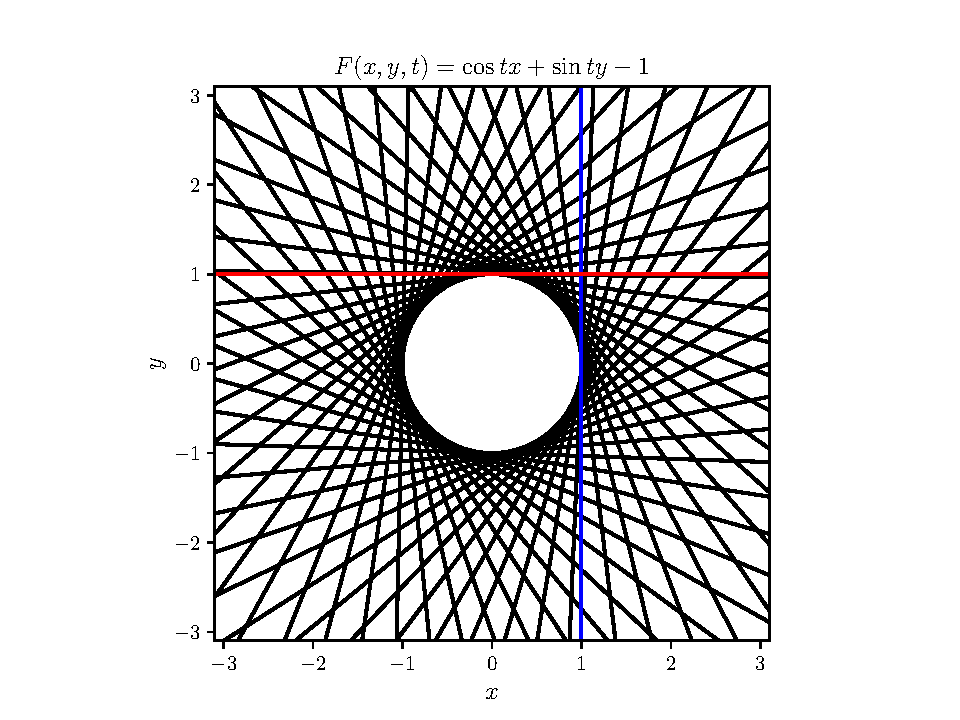
\includegraphics{images/lines_in_normal_form.pdf}
	\caption{Systém priamok v normálovom tvare.}
	\label{fig:lines_in_normal_form}
\end{figure}

\end{example}

Transformácie $g_{t}$ z príkladu sú prvkami Lieovej grupy $SO(n)$. Ďalšie známe príklady maticových Lieovych grúp sú ortogonálna grupa $O(n)$, unitárna $U(n)$ a špeciálna unitárna grupa $SU(n).$ 
Pre nájdenie podrobnejších informácií, sa môže čitateľ obrátiť na ľubovoľnú úvodnú učebnicu o Lieovych grupách a Lieovych algebrách, ako je napríklad \cite{Lee12}.
Použili sme štruktúru Lieovej grupy, aby sme opísali, ako sa grupa transformuje daný povrch. Ďalej, využijúc štruktúru hladkej variety môžeme opísať jednoparametrický systém plôch výlučne pomocou terminológie Lieových grúp. Táto teória sa aplikuje na nájdenie parametrizácie obálok kvadratických plôch. Viac o tomto prístupe možno nájsť v \cite{Vra22}. 

\subsection{Obálky a ODR}
Obálky súvisia aj so štúdiom obyčajných diferenciálnych rovníc, a najmä ich singulárnych riešení. Predpokladajme, že jednoparametrický systém kriviek $\mathcal{F}_t$ je riešením nejakej diferenciálnej rovnice prvého rádu. Potom môže existovať aj ďalšia krivka spĺňajúca túto diferenciálnu rovnicu, ktorá je dotyčnicou k $\mathcal{F}_t$ v každom bode. Táto krivka je obálka. V literatúre sa nazýva aj singulárne riešenie diferenciálnej rovnice.
Uvažujme ODR 
$$
\left(\frac{dy}{dx}\right)^2 - 4x\frac{dy}{dx} + 4y = 0.
$$
Jej regulárnym riešením sú integrálne krivky 
$$ y = - t^2 + 2tx, \text{ kde } t \in \mathbb{R}.$$
Riešenie môžeme reprezentovať ako jednoparametrický systém kriviek $\mathcal{F}_t$ s funkciou
$$F(x,y,t) = t^2 - 2tx + y. $$
Derivovaním podľa parametra $t$ dostávame
$$\dfrac{\partial F}{\partial t} (x,y,t) = 2t - 2x, $$
z čoho máme $t=x$ a dosadením do funkcie máme $F=-x^2+y,$ teda obálka je $y=x^2.$

Obálka tejto jednoparametrickej rodiny priamok, ktorou je parabola $y = x^2$, rieši taktiež diferenciálnu rovnicu. Viac o tomto prístupe možno nájsť v \cite{Gro97}.

\begin{figure}[H]
	\centering
	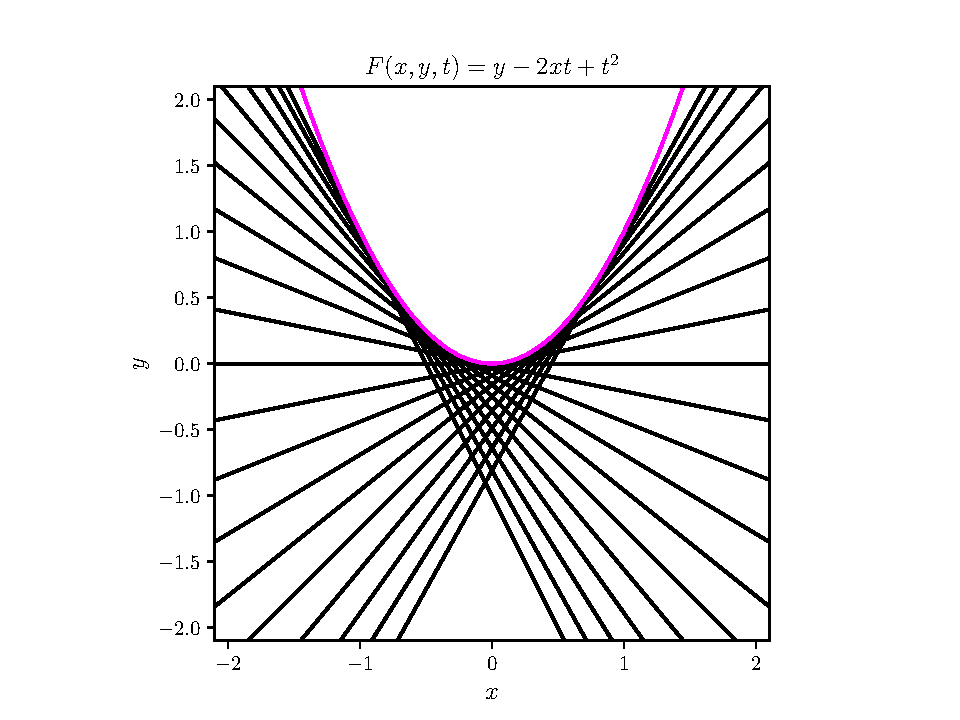
\includegraphics{images/odr.pdf}
	\caption{Regulárne riešenia a obálka.}
	\label{fig:odr}
\end{figure}

\subsection{Lokálne prieniky} \label{lokalne prieniky pre krivky}
Lokálny prienik systému kriviek $\mathcal{F}_t $ pozostáva z prienikov blízkych susedných kriviek systému. Tento koncept bude ďalej formálne definovaný.
\begin{definition}[Lokálny priesečník]
Lokálny priesečník systému $\mathcal{F}_t$ je množina všetkých priesečníkov infinitezimálne blízkych prvkov pre $t$. Označuje sa ako $\mathcal{L}$ a formálne platí
$$
\mathcal{L}_{t_0} = \lim_{\varepsilon \to 0} \mathcal{F}_{t_0} \cap \mathcal{F}_{t_0 + \varepsilon}.
$$
Lokálny priesečník $\mathcal{L} := \bigcup_{t \in I} \mathcal{L}_{t}$ systému $\mathcal{F}_t $ je zjednotenie všetkých priesečníkov vzniknutých z takýchto prekrytí.
\end{definition}
Lokálny priesečník regulárneho systému sa v mnohých prípadoch zhoduje s jeho obálkou. Ilujstrujme to na nasledovnom príklade.

\begin{example}
Vezmime dva ľubovoľné, ale odlišné prvky systému $F(x, y, t) = y - 2tx - t.$
Pre fixné parametre $t_1 \neq t_2$ tak máme
$$F(x_1, y_1, t_1) = y_1 - 2t_1x_1 - t_1^2,$$
$$F(x_2, y_2, t_2) = y_2 - 2t_2x_2 - t_2^2.$$ 
Označme priesečník týchto dvoch priamok $Q = (q_x, q_y)^T.$ Pre priesečník $Q$ platí $$F(q_x, q_y, t_1) = 0 = F(q_x, q_y, t_2),$$ odkiaľ vyplýva 
$$(t_2 - t_1)(2q_x + t_1 + t_2) = 0.$$ 
Keďže podľa predpokladu $t_1 \neq t_2$, jediné riešenie tejto rovnice je $q_x = -\dfrac{t_1 + t_2}{2}$ a priesečník je potom daný 
$$Q = (-\dfrac{t_1 + t_2}{2}, -t_1t_2)^T.$$ Definujme $\varepsilon := t_2 - t_1$ a nechajme $\varepsilon$ smerovať k nule, dostávame priesečník
$$
\lim_{\varepsilon \to 0} 
\begin{pmatrix} 
-t_1 - \dfrac{\varepsilon}{2} \\
-t_1(t_1 + \varepsilon)
\end{pmatrix} = \begin{pmatrix} 
-t_1 \\
-t_1^2
\end{pmatrix}.
$$
Po reparametrizácii $t_1(t) = -t$ je ľahké vidieť, že množina všetkých týchto priesečníkov $\mathcal{L} = \{(t, -t^2): t \in \mathbb{R}\} = \mathcal{E}$, ktorá predstavuje lokálny priesečník, sa zhoduje s vypočítanou množinou bodov obálky.
\end{example}

\begin{corollary} Nech je daný systém $\mathcal{F}$. Potom každý bod lokálneho priesečníka systému $\mathcal{L}$ je aj bodom obálky systému $\mathcal{E}$. Teda platí
$$ \mathcal{L} \subseteq \mathcal{E}. $$
\end{corollary}

\section{Aplikácie obálok a predošlá práca}
Vzhľadom na výskyt obálok v aplikáciách sa obálkam venuje veľká pozornosť. Stručne spomenieme niektoré aplikácie a odkážeme na literatúru. 

Výpočet obálky pohybujúcej sa plochy sa vyskytuje pri simulácii a CNC obrábaní. CNC obrábanie \textit{(Computer Numerical Control machining)}  je výrobný subtraktívny proces, pri ktorom počítač riadi stroje, napríklad vŕtačky, frézy a sústruhy tak, aby neustále odlamovali nadbytočnosti z obrobku. Tento postup sa vykonáva, kým sa nevytvorí požadovaný tvar. Rezný nástroj vytvára pri rýchlom otáčavom pohybe okolo svojej osi rotačnú plochu. Takto vytvorená plocha je časť obálky pohybujúceho sa nástroja. CNC frézovanie má široké priemyselné využitie v odvetviach ako letecký priemysel, zdravotníctvo a spotrebná elektronika. V článku \cite{Skop20} sa možno dočítať viac o výpočte obálok pri 5-osovom CNC obrábaní.  

Obálky sa používajú aj na výpočet trajektórie projektilu vo vzduchu. Riešime klasický problém pohybu hmotného bodu (projektilu) vrhaného pod uhlom k horizontu. S nulovou silou odporu vzduchu je analytické riešenie dobre známe, trajektória projektilu je parabola. So zohľadnením odporu vzduchu úloha nemá presné analytické riešenie, a preto sa vo väčšine prípadov rieši numericky. Silu odporu vzduchu berieme do úvahy s konštantným členom odporu. Systém trajektórií vzniká pri vrhnutí projektilu s rovnakou počiatočnou rýchlosťou, ale s rôznymi uhlami hodu. Na určenie maximálneho rozsahu letu projektilu sa tak použije rovnica obálky. \cite{Chud09}

%krivka s kontrolou chyby (Wallner)
Medzi ďalšie aplikácie obálok patrí tollerancing – krivka s kontrolou chyby, bezkolízne plánovanie pohybu robota – uvažujeme o konvexných kompaktných krivkách reprezentujúcich pohyb robota v rovine, ktorý mení svoj lokálny tvar pomocou systému afinných transformácií. Dizajn písma – konštrukcia znakov v písmach pre typografické systémy. O ďalších aplikáciach sa čitateľ dozvie v \cite{Pott09}.

Kanálové plochy \textit{(channel surfaces)}, rúrkové plochy/potrubia \textit{(pipe surfaces}), \textit{rolling ball blends} a prirodzené kanálové plochy \textit{(natural channel surfaces)} sa vyskytujú ako zmiešavacie povrchy a prechodové plochy medzi potrubiami. Kanálové plochy sú používané v počítačom podporovanom geometrickom dizajne \textit{(Computer Aided Geometric Design)}. V ďalšom texte si ukážeme ich konštrukciu ako obálku sfér.

Obálky - kanálové plochy sa využívajú aj v architektúre. Ako príklad uvádzame Webbov most \textit{(Webb Bridge)}, obr. \ref{fig:webb_bridge} v Melbourne v Austrálii. Tvar mosta vzdáva hold histórii domorodého obyvateľstva a je vytvorený podľa tradičnej rybárskej pasce Koorie, ktorá sa používala na lov úhorov.

\begin{figure}[h!]
	\centering
	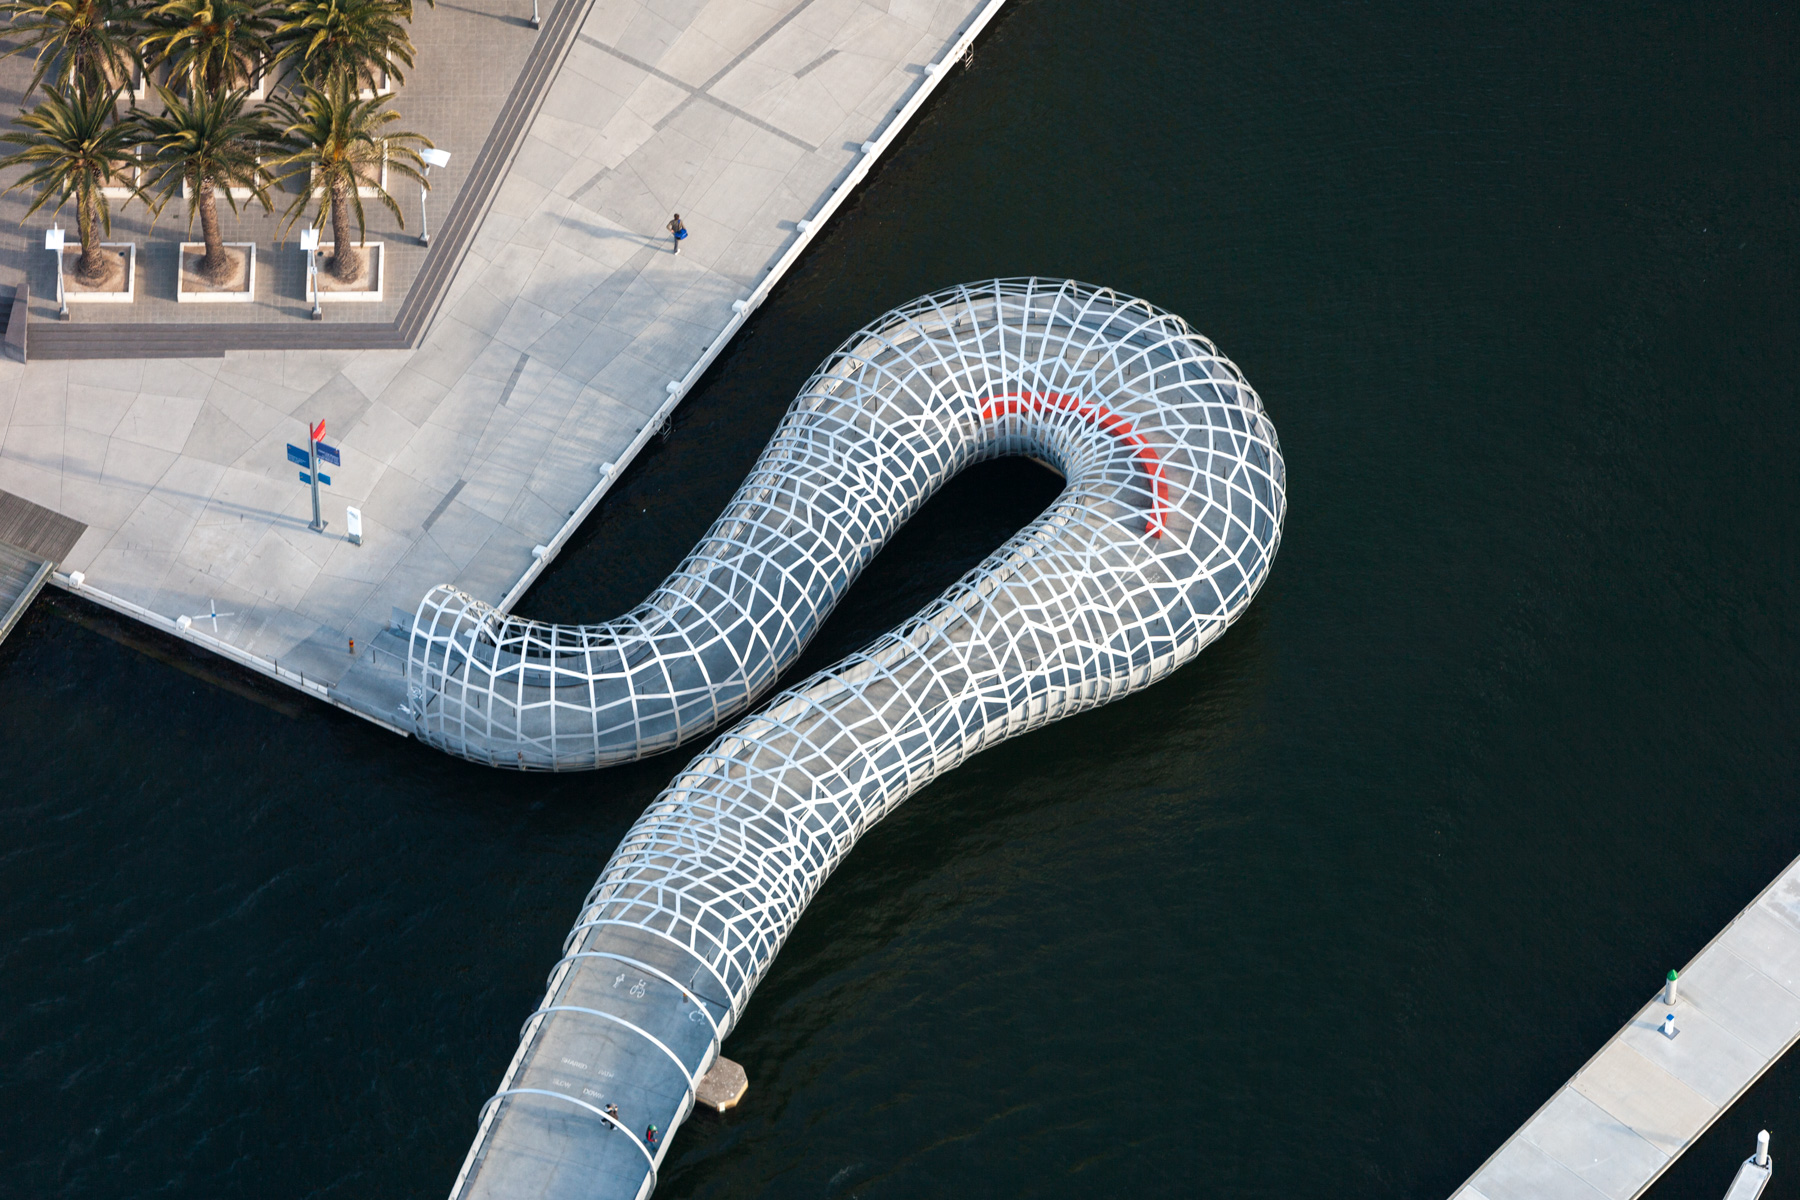
\includegraphics[width=\textwidth]{images/webbbridge.jpg}
	\caption[Webbov most.]{Webbov most. \cite{WebbBridge}}
	\label{fig:webb_bridge}
\end{figure}

\section{Obálka sfér}
Označme $Q \in \mathbb{R}^3$ a predpokladajme, že $m(t) = (m_1(t), m_2(t), m_3(t)) \colon I \subset \mathbb{R} \rightarrow \mathbb{R}^3$ je parametrizácia krivky $m$ a $r(t) \colon I \rightarrow \mathbb{R}^{+}$ je funkcia definovaná na tom istom intervale. Krivka $m$ sa nazýva kostrová krivka obálky (\textit{spine curve}) a $r$ sa nazýva funkcia polomeru (\textit{radius function}). Jednoparametrický systém sfér je daný rovnicou

$$
\mathcal{S}_t \colon \langle Q - m(t), Q - m(t) \rangle - r^2(t)= 0.
$$

Podľa definície \ref{charakterizacia}, obálku $\mathcal{E}$ možno nájsť ako prienik $\mathcal{S}_t$ a $\mathcal{\dot{S}}_t$ pre všetky $t \in I$. Derivácia $\mathcal{S}$ nám dáva roviny

$$
\mathcal{\dot{S}}_t \colon \langle \dot{m}(t), Q - m(t) \rangle + r(t) \dot{r}(t) = 0.
$$

Budeme teda hľadať prieniky sféry a roviny pre každý parameter $t \in I$.

\subsection{Charakteristická kružnica}
\begin{definition}[Charakteristická kružnica]
V prípade, že pre $t_0 \in I$ je $\mathcal{S}_{t_0} \cap \mathcal{\dot{S}}_{t_0} \neq \emptyset$, sa tento prienik nazýva sa charakteristická kružnica $c_{t_0}$. V prípade $\mathcal{S}_{t_0} \cap \mathcal{\dot{S}}_{t_0} = \emptyset$, pre \(t_0\) neexistuje žiadna charakteristická kružnica.
\end{definition}

\begin{lemma} \label{lema o zjednoteni charakteristickych kruznic}
Zjednotenie všetkých charakteristických kružníc $c_t$ jednoparametrického systému $\mathcal{S}_t$ je obálka $\mathcal{E}$ tohto systému, teda platí $$\mathcal{E} = \bigcup_{t \in I} c_t.$$
\end{lemma}

\begin{proof}
Nech bod $Q$ patrí do zjednotenia kružníc $ \bigcup_{t \in I} c_t, $ potom existuje aspoň jedno $t_0 \in I, $ pre ktoré $Q \in c_{t_0}.$ Keďže $c_{t_0} = \mathcal{S}_{t_0} \cap \mathcal{\dot{S}}_{t_0}, $ tak sú rovnice $\mathcal{S}_{t_0} $ a $ \mathcal{\dot{S}}_{t_0}$ splnené pre nejaké $t_0$ a $Q,$ a preto patrí $Q$ obálke $\mathcal{E}, $ a teda platí inklúzia $\bigcup_{t \in I} c_t \subseteq \mathcal{E}. $

Opačne, ak $Q$ patrí obálke $\mathcal{E},$ existuje podľa definície \ref{charakterizacia} $t_0 \in I $ také, že platí $F(Q,t_0) = 0$ a súčasne $\dfrac{\partial F}{\partial t}(Q, t_0)=0,$ to znamená, že $Q$ leží v prieniku $\mathcal{S}_{t_0} \cap \mathcal{\dot{S}}_{t_0} = c_{t_0} $ a $c_{t_0} \subseteq \bigcup_{t \in I} c_t. $ Preto platí inklúzia $\mathcal{E} \subseteq \bigcup_{t \in I} c_t.$ 

Týmto je rovnosť $\mathcal{E} = \bigcup_{t \in I} c_t$ dokázaná.
\end{proof}

Obálka sfér sa teda skladá zo systému kružníc. Charakteristická kružnica leží celá v rovine $\mathcal{\dot{S}}_t $, takže v tejto rovine leží aj jej stred. Dotykový vektor kostrovej krivky $m(t)$ je kolmý na rovinu $\mathcal{\dot{S}}_t$, teda stred $C_t$ charakteristickej kružnice leží na dotyčnici $T(t, s)= m(t) + s \cdot \dot{m}(t), s \in \mathbb{R}$, preto stred $C_t$ nájdeme ako
$$ \mathcal{\dot{S}}_t \cap T(t, s).$$
Pre parameter $s$ potom platí $s = \dfrac{r(t) \dot{r}(t)}{\langle \dot{m}(t), \dot{m}(t) \rangle }, $
po dosadení do $T(t, s)$ získavame
\begin{equation}
\label{eq:stred charakteristickej kruznice}
C_t = m(t) - \frac{r(t) \dot{r}(t)}{\langle \dot{m}(t), \dot{m}(t) \rangle} \dot{m}(t).
\end{equation}

Rozoberme si nasledujúce dva prípady
\begin{itemize}
\item Ak je funkcia polomeru $r(t)$ konštantná, $\dot{r} \equiv 0$ a rovina $\mathcal{\dot{S}}_t$ obsahuje stred sféry $M_t$ pre všetky $t \in I$, v tomto prípade možno obálku $\mathcal{E}$ považovať za posunutie (\textit{offset}) kostrovej krivky $m$. Tieto obálky sú známe ako rúrkové plochy (\textit{pipe surfaces}). Keďže rovina $\mathcal{\dot{S}}_t$ charakteristickej kružnice $c_t$ obsahuje stred sféry $M_t$ v každom $t \in I$, charakteristická krivka je hlavnou kružnicou sféry a obálka $\mathcal{E}$ je pokrytá jednoparametrickým systémom zhodných kružníc.
\item Ak funkcia polomeru $r(t)$ nie je konštantná, potom $\dot{r}(t) \neq 0$ a rovina $\mathcal{\dot{S}}_t$  neprechádza stredom sféry $M_t$. V tomto prípade obálka $\mathcal{E}$ patrí do triedy kanálových plôch.
\end{itemize}

Polomer $l_t$ charakteristiskej kružnice  možno vypočítať z pravouhlého trojuholníka $M_tC_tP,$ kde $P$ je ľubovoľný bod na charakteristickej kružnici $c_t$, a teda aj na sfére $\mathcal{S}_t.$
$$ l_t = \sqrt{r^2(t) - \|M_tC_t\|^2} = r(t) \sqrt{ 1 - \frac{\dot{r}^2(t)}{\langle \dot{m}(t), \dot{m}(t) \rangle}}. $$
V prípade, že $ \|M_tC_t\| > r(t)$, sféra $S$ nemá s obálkou $\mathcal{E}$ reálny kontakt. 

\begin{example}
Uvažujme kostrovú krivku $m(t)$ a polomer $r(t)$
$$ 
m(t) = \begin{pmatrix} 0 \\ 0 \\ t \end{pmatrix} \quad \text{ a } \quad r(t) = \frac{t}{\sqrt{26}}.
$$
potom obálka systému je daná rovnicami
\begin{align*}
&\mathcal{S}_t \colon x^2 + y^2 + (z - t)^2 - \frac{t^2}{26} = 0, \\
&\mathcal{\dot{S}}_t \colon z - \frac{25}{26}t = 0. \\
\end{align*}
Počítajme $ \mathcal{S}_t \cap \mathcal{\dot{S}}_t $ pre všetky $t \in \mathbb{R}.$ Z druhej rovnice dostaneme $t = \frac{26}{25}z$. Po dosadení do prvej rovnice, dostávame implicitnú rovnicu pre obálku $\mathcal{E}$
$$
x^2 + y^2 - \frac{1}{25}z^2 = 0,
$$
čo je rovnica rotačného kužeľa.

Napríklad, pre $t = 1 \in I$ charakteristická krivka je prienikom dvoch plôch daných
\begin{align*}
&\mathcal{S}_1 \colon x^2 + y^2 + (z - 1)^2 - \frac{1}{26} = 0, \\
&\mathcal{\dot{S}}_1 \colon z - \frac{25}{26} = 0. \\
\end{align*}
Z toho môžeme usúdiť, že charakteristická krivka $c_1$ je kružnica so stredom v bode $C_1 = (0, 0, \frac{25}{26})$ v rovine $z = \frac{25}{26}$ a neprechádza stredom sféry $M_1 = m(1) = (0,0,1)$, polomer $c_1$ je $l_{1} = \frac{\sqrt{25}}{26}$. Vzdialenosť bodov $ \|M_tC_t\| = \frac{1}{26}$ a $r(1)= \frac{1}{\sqrt{26}}$, takže platí, že $r(1) > \|M_tC_t\|$ a sféra $\mathcal{S}_1$ má s obálkou $\mathcal{E}$ reálny kontakt.
\end{example}

Jedným z dôležitých výsledkov je, že kanálové plochy, definované ako obálka jednoparametrického systému sfér s racionálnou funkciou polomeru $r(t)$ a stredmi v racionálnej krivke $m(t)$ možno racionálne parametrizovať. \cite{Pet97}

Bohužiaľ, vo väčšine prípadov sú rovnice, ktoré charakterizujú obálky, príliš zložité a odvodiť z nich rovnicu obálky nie sme schopní.

Rúrkové povrchy sa často objavujú pri výrobe potrubia. Hladké spojenie medzi dvoma nie nevyhnutne valcovými rúrami $P_1$ a $P_2$ sa modeluje tak, aby bol prechod hladký, bez záhybov, vodotesný alebo dokonca aj parotesný. Na to sa používa technika \textit{rolling ball blends}, využívajúca nasledujúcu myšlienku: Kým sa sféra $S$ s konštantným alebo nekonštantným polomerom $r$ kotúľa na oboch rúrach súčasne, zanecháva stopu $c_i$ na oboch rúrach. Zmiešavacia plocha je tá časť obálky $\mathcal{E}$ jednoparametrického systému sfér, ktorá leží medzi dvoma stopami $c_1$ a $c_2$. Kostrová krivka obálky $\mathcal{E}$ je priesečníkom ekvidištánt \textit{(offsetov)} plôch $P_1$ a $P_2$ vo vzdialenosti $r$. Každá charakteristická krivka spája dva dotykové body zmiešavacej plochy a plochami $P_1$ a $P_2$, ktoré sa majú zmiešavať. Viac detailov možno nájsť v \cite{Kar00} a \cite{Ode20}. Na obrázku \ref{fig:rolling_ball_blends} vľavo je znázornená metóda so sférou s konštantným polomerom $r$, vpravo s nekonštantným.

\begin{figure}[H]
	\centering
	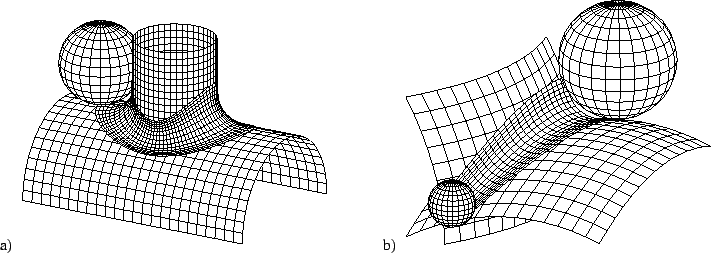
\includegraphics[width=\textwidth]{images/rolling_ball_blends.png}
	\caption[Technika rolling ball blends.]{Technika rolling ball blend s konštatným polomerom vľavo, s nekonštantným polomerom vpravo. \cite{Rollingballblends}}
	\label{fig:rolling_ball_blends}
\end{figure}

\subsection{Lokálny prienik}
V časti \ref{lokalne prieniky pre krivky} sme odvodili vzťahy medzi lokálnym prienikom jednoparametrického systému a jeho obálkou. Pre systém kružníc však platí viac ako inklúzia jedným smerom.

\begin{lemma} \label{lema o lokalnom prieniku sfer}
Lokálny prienik $\mathcal{L}_{t_0}$ jednoparametrického systému sfér $\mathcal{S}_t$ pre $t_0 \in I$ zodpovedá charakteristickej kružnici $c_{t_0}$. Platí $$
\mathcal{L}_{t_0} = c_{t_0}.
$$
\end{lemma}

\begin{proof}
Ukážeme, že lokálny prienik dvoch nekonečne blízkych sfér $\mathcal{S}_{t_1}$ a $\mathcal{S}_{t_2}$ pre $\varepsilon = t_2 - t_1$ idúce k nule, bude práve charakteristická kružnica $c_{t_2}$ a to tak, že pomocou orientovanej vzdialenosti stredov sfér ukážeme, že stred charakteristickej kružnice a stred prieniku dvoch sfér sú rovnaké.
Označme ľubovoľný bod $S \in \mathcal{S}_{t_1} \cap \mathcal{S}_{t_2}, l $ vzdialenosť medzi bodmi $S$ a $C$ a $\vec{t} $ bude jednotkový vektor v smere $ m(t_2) - m(t_1).$
Označme ako $d_1$ orientovanú vzdialenosť $m(t_1)$ a $C$ a podobne $d_2$ orientovanú vzdialenosť $m(t_2)$ a $C.$
$$ d_1 = \langle \vec{t}, C - m(t_1) \rangle \quad d_2 = \langle m(t_2) - C,  \vec{t} \rangle, $$
kde $d_1 + d_2 = | m(t_2) - m(t_1) |.$

Keďže $m(t_2)CS$ a $m(t_1)CS$ sú pravouhlé, môžeme vyjadriť dĺžku spoločnej odvesny $l.$
$$l^2 = r^2(t_1) - d^2_1 = r^2(t_2) - d^2_2,$$
kde $d_2 = |m(t_2) - m(t_1)| - d_1, $
potom možno $d_1$ vyjadriť ako 
$$d_1 = \dfrac{ | m(t_2) - m(t_1) |}{2} - \dfrac{\dfrac{r(t_2)-r(t_1)}{t_2-t_1} (r(t_2) +r(t_1))}{\dfrac{ | m(t_2)-m(t_1) |}{t_2 - t_1}}.$$
Pre $\varepsilon = t_2 - t_1 $ idúce k nule
$$ d_1 = - \dfrac{\dot{r}(t_1) r(t_1)}{| \dot{m}(t_1) |}.  $$
Odkiaľ stred priesečníkovej kružnice je
$$S = m(t) + d_t \dfrac{\dot{m}(t)}{| \dot{m}(t)|} = m(t) - \dot{m}(t)\dfrac{r(t)\dot{r}(t)}{|\dot{m}(t)|}. $$
Tento stred $S$ zodpovedá rovnici \ref{eq:stred charakteristickej kruznice} pre stred $C_t$ charakteristickej kružnice $c_t$. Nekonečne blízke sféry sa pretínajú pre $t_0$ v rovine $\mathcal{\dot{S}}_{t_0}$, a preto je prienik daný ako 
$$ \mathcal{L}_{t_0} = \mathcal{S}_{t_0} \cap \mathcal{\dot{S}}_{t_0} = c_{t_0}. $$
V prípade, že lokálny prienik $\mathcal{L}_{s}$ pre nejaké $s \in I$ prázdny, neexistuje pre $s$ žiadna charakteristická kružnica a uvedená rovnosť stále platí.
\end{proof}

\begin{theorem}
Obálka $\mathcal{E}$ jednoparametrického systému sfér $\mathcal{S}_t$ pozostáva z bodov prieniku infinitezimálne blízkych prvkov systému a platí $$
\mathcal{L} = \mathcal{E}.
$$
\end{theorem}

\begin{proof}
Z predchádzajúcich dvoch lem, lemy \ref{lema o zjednoteni charakteristickych kruznic} a \ref{lema o lokalnom prieniku sfer} platí 
$$ \mathcal{E} = \bigcup_{t \in I } c_t = \bigcup_{t \in I} \mathcal{L}_t = \mathcal{L}. $$
\end{proof}

\subsection{Lokálny samoprienik}
Lokálny samoprienik obálky jednoparametrického systému guľových plôch je špeciálnym typom samopretínania obálky. Je definovaný nasledovne.
\begin{definition} \label{definicia lokalny samoprienik}
Lokálny samoprienik $\mathcal{L}_{t_0}$ obálky $\mathcal{E}$ pre $t_0$ je priesečníkom infinitezimálne blízkych charakteristických kružníc $c$ systému $\mathcal{F}$. Lokálny samoprienik obálky je množina všetkých priesečníkov, ktoré vznikajú z takýchto prekrývaní. Označíme ho ako $\mathcal{L} = \bigcup_{t \in I} \mathcal{L}_t$.
\end{definition}

Nasledujúci výrok predstavuje dôležité kritérium na identifikáciu lokálneho samoprieniku.
\begin{lemma} \label{kriterium o lokalnom samoprieniku}
Bod $Q \in \mathbb{R}^3$ patrí práve vtedy do lokálneho samoprieniku $\mathcal{L}_{t_0}$ obálky $\mathcal{E}$, ak sú splnené rovnice
\begin{align*}
F(Q,t_0) &= 0, \\
\dfrac{\partial F}{\partial t}(Q,t_0) &= 0, \\
\dfrac{\partial^2 F}{\partial t^2}(Q,t_0) &= 0
\end{align*}
pre nejaké $t_0 \in I.$
\end{lemma}

\begin{proof}
Ľubovoľný bod $Q \in \mathcal{L}_{t_0}$ patrí podľa definície k priesečníku infinitezimálne blízkych kruhov pre $t_0$. V bode $Q$ sa navzájom pretínajú aj roviny $\mathcal{\dot{S}}_t$, v ktorých sa tieto kružnice nachádzajú. Tieto roviny patria do systému $\mathcal{\dot{S}}$, ktorá je definovaná ako množina nulových bodov funkcie $\dfrac{\partial F}{\partial t}(Q, t_0)$, a sú tiež infinitezimálne blízko, to znamená, že platí $\dfrac{\partial^2 F}{\partial t^2}(Q,t_0) = 0, $ teda
\begin{equation}
\label{eq:druha derivacia}
\langle \ddot{m}(t_0), Q-m(t_0) \rangle - \langle \dot{m}(t_0), \dot{m}(t_0) \rangle + \dot{r}^2(t_0) + r(t_0)\ddot{r}(t_0) = 0. 
\end{equation}
Bod $Q$ leží na charakteristickej kružnici $c_{t_0},$ preto spĺňa rovnice $F $ a $\dfrac{\partial F}{\partial t}.$ Toto je nutná podmienka.

Opačne, predpokladajme, že sú všetky rovnosti z tejto lemy splnené pre nejaké $t_0 \in I$ a $Q \in \mathbb{R}^3, $ potom platí
\begin{align*}
Q &\in \lim_{\varepsilon \to 0} \left( \mathcal{S}(t_0) \cap \mathcal{S}(t_0 + \varepsilon) \cap  \mathcal{\dot{S}}(t_0) \cap  \mathcal{\dot{S}}(t_0 + \varepsilon) \right) \\
&= \lim_{\varepsilon \to 0} \left( \underbrace{\mathcal{S}(t_0) \cap \mathcal{\dot{S}}(t_0)}_{c_{t_0}} \cap \underbrace{\mathcal{S}(t_0 + \varepsilon) \cap \mathcal{\dot{S}}(t_0 + \varepsilon)}_{c_{t_0 + \varepsilon}} \right) \\
&= \lim_{\varepsilon \to 0} \left( {c_{t_0}} \cap {c_{t_0 + \varepsilon}} \right) \\
&= \mathcal{L}_{t_0}.
\end{align*}
Týmto sme ukázali, že bod $Q$ patrí do samoprieniku charakteristických kružníc pre $t_0$ a podľa definície \ref{definicia lokalny samoprienik} patrí do lokálneho samoprieniku $\mathcal{L}_{t_0}$ obálky $\mathcal{E}$.
\end{proof}

Pomocou lemy \ref{kriterium o lokalnom samoprieniku} možno ľahko rozhodnúť, či bod $Q \in \mathbb{R}^3$ pre parameter $t_0 \in I$ patrí do lokálneho samoprieniku $\mathcal{L}_{t_0}.$ Ak je $t_0$ neznáme, mohli by sme určiť $t_i$ z rovnice $\dfrac{\partial^2 F}{\partial t^2}$. Ak by pár $(Q, t_i)$ spĺňal obe ďalšie rovnice, bod $Q$ patrí do lokálneho samoprieniku obálky $\mathcal{E}$ pre $t_i.$

Často však riešime otázku, či obálka má lokálny samoprienik a ak áno, pre aké hodnoty parametrov $t \in I$. Pre túto otázku nie je použitie lemy \ref{lema o lokalnom samoprieniku} vhodné, preto predkladáme lepšie kritérium. Pozrieme sa na to z geometrického hľadiska. Rovnica \ref{eq:druha derivacia} definuje systém rovín $\mathcal{\ddot{S}}_t$. Pre každé $t \in I$ je vektor $\ddot{c}(t)$ kolmý na $\mathcal{\ddot{S}}_t.$ Prvé dve rovnice z lemy \ref{eq:druha derivacia} definujú pre pevné $q \in I$ charakteristickú kružnicu $c_q$, to znamená, že pre $q$ existuje lokálny samoprienik $\mathcal{L}_q$, ak sa $c_q$ a $\mathcal{\ddot{S}}_q$ pretínajú. 

Keďže roviny $\mathcal{\dot{S}}$ aj $\mathcal{\ddot{S}}$ sú rovnobežné s vektorom $ \vec{\dot{m}}(q) \times \vec{\ddot{c}(q)} $, môžu byť obe roviny projektované do roviny obsahujúcej $ c(q) $ a kolmej na $ \vec{b}_q $ a problém priesečníka môžeme takto vyriešiť. Pod $ \vec{b}_q $ sa rozumie binormálový vektor definovaný v bode krivky $ c(q) $. Nech $\vec{n}(q)$ je zodpovedajúci normálový vektor. Označme prienik priamok $C_q + s \cdot \vec{n}_q$, $s \in \mathbb{R}$, s rovinou $\mathcal{\ddot{S}}_t$ ako $S_t = C_q + s_t \cdot \vec{n}_q$ s prislúchajúcim parametrom $s_t$. Bod $S_t$ lokálneho prieniku pre $q$ existuje, ak jeho vzdialenosť od stredu $C_t$ charakteristickej kružnice $c_t$ je menšia ako jej polomer $l_t.$ 

\begin{align*}
| S_t - C_t | &= | s_t \cdot \vec{n}_t | = | s_t | \leq l_t.
\end{align*}

Toto je ďalšie kritérium pre existenciu lokálneho prieniku. Na určenie parametra priesečníka $ s $ sa pozrieme na nasledovnú rovnicu. Do rovnice \ref{eq:druha derivacia} dosadíme vyjadrenie pre bod prieniku.

\begin{align*}
\langle \ddot{m}(t), C_t + s_t \cdot \vec{n}(t) - m(t) \rangle - \langle \dot{c}, \dot{c}\rangle + \dot{r}^2(t) + r(t)\ddot{r}(t) = 0
\end{align*}

Odkiaľ pre parameter $ s_t $ dostávame vyjadrenie

\begin{align*}
s_t &= \dfrac{ r(t) \dot{r}(t) \langle \dot{m}(t), \ddot{m}(t) \rangle + \langle \dot{m}(t), \dot{m}(t) \rangle^2 - \left( \dot{r}^2(t) + r(t)\ddot{r}(t) \right) \langle \dot{m}(t), \dot{m}(t) \rangle}{\langle \dot{m}(t), \dot{m}(t) \rangle \langle \ddot{m}(t) , \vec{n}(t) \rangle}.
\end{align*}

Tento výraz je síce dosť zložitý, avšak umožňuje identifikovať intervaly parametra $ t $, v ktorých existuje lokálny priesečník obálky $ \mathcal{E} $ prostredníctvom nájdenia koreňov funkcie $ g(t) = | s_t | - l_t $. Samotné priesečníky pre to však nemusia byť známe.

\textit{Pozorovanie:}
Pomocou kritéria je samozrejme možné efektívne rozhodnúť o tom, či sa obalová plocha lokálne pretína v určitom parametri $t_0 \in I$ bez toho, aby sme poznali priesečníky bodov. Tie sa potom dajú ľahko určiť pomocou
$$
S_{\pm} = C_{t_0} + s_{t_0} \cdot \vec{n}_{t_0} + b_{\pm} \cdot \vec{b}_{t_0},
$$
kde $ b_{-} \in \mathbb{R} $ a $ b_{+} \in \mathbb{R} $ a $s_t^2 + b_{\pm}^2 = l_t^2 $ z pravouhlých trojuholníkov $C_{t_0}S_{-}S_{t_0}$ a $C_{t_0}S_{+}S_{t_0}$

\subsection{Konštantný polomer}
V prípade, že je funkcia polomeru $r(t) \equiv r $ konštantná, platí $C_t = M_t,  l_t = r$ a $\dot{r} = 0,$ preto 
$$\dfrac{\partial^2 F}{\partial t^2} = s \cdot \langle \ddot{c}(t), n(t) \rangle - \langle \dot{c}(t), \dot{c}(t) \rangle = 0$$
a kritérium pre existenciu lokálneho prieniku $\mathcal{L}_t$ sa zjednoduší na
$$
\lvert s \rvert = \frac{\langle \dot{c}(t), \dot{c}(t) \rangle}{\langle \ddot{c}(t), n(t) \rangle} \leq r.
$$
\begin{example}
Pre prípad, že stredová krivka je daná normálnou parabolou, platí pre jej parametrizáciu a derivácie

\[
m(t) = \begin{pmatrix} t \\ t^2 \\ 0 \end{pmatrix}, \quad \dot{m}(t) = \begin{pmatrix} 1 \\ 2t \\ 0 \end{pmatrix} \quad \text{a} \quad \ddot{m}(t) = \begin{pmatrix} 0 \\ 2 \\ 0 \end{pmatrix}.
\]
Z toho ľahko získame vektory 
$$ \dot{m}(t) \times \ddot{m}(t) =
\begin{pmatrix} 0 \\ 0 \\ 2 \end{pmatrix} , \quad \vec{b}(t) = \begin{pmatrix} 0 \\ 0 \\ 1 \end{pmatrix} \quad  \text{a} \quad \vec{n}(t) = \dfrac{1}{\sqrt{4t^2 + 1}} \begin{pmatrix} -2t \\ 1 \\ 0 \end{pmatrix}.$$
Ak je polomer konštantný, dostávame pre parameter samoprieseku
$$ s_t = \dfrac{\sqrt{4t^2 + 1}^3}{2}, $$
ktorý je rovný obrátenej hodnote krivosti krivky $m(t)$ a to
$$ \kappa(t) = \frac{\lVert  \dot{m}(t) \times \ddot{m}(t) \rVert}{\lVert \dot{m}(t) \rVert^3} = \frac{2}{\sqrt{4t^2 + 1}^3}. $$
Zrejme platí, že $s_t$ je vždy väčšie alebo rovné $\frac{1}{2}$. To znamená, že pre všetky polomery $r < \frac{1}{2}$ neexistuje žiadny lokálny prienik. Väčšie polomery vedú k lokálnemu pretínaniu obálky pre hodnoty parametrov $t$ v intervale $[-a; a]$ s $a \in \mathbb{R}^+ \setminus {0}$. Napríklad pre $r = 1$ platí $a = \frac{1}{2} \sqrt{2 \sqrt{3} - 1} \approx 0.38$.
\end{example}

Vzťah medzi krivosťou a parametrom priesečníka neplatí len pre tento konkrétny príklad, ale vo všeobecnosti.

\begin{lemma}
Pre obálku $\mathcal{E}$ jednoparametrického systému sfér $\mathcal{S}_t$ s konštantným polomerom $r(t) \equiv r \in \mathbb{R}$ je splnená rovnosť 
$$ s_t = \dfrac{1}{\kappa(t)} $$
pre všetky $t \in I$, kde $\kappa$ je krivosť kostrovej krivky $m(t).$
\end{lemma}

\begin{proof}
Označme $\alpha_t $ uhol medzi $m(t)$ a $\dot{m}(t)$ a $\beta_t $ uhol medzi $n(t)$ a $\ddot{m}(t)$. Potom platí $\alpha_t = 90 - \beta_t$ alebo $\alpha_t = 90 + \beta_t$. V oboch prípadoch je $\sin (\alpha_t) = \cos (\beta_t).$ Počítajme veľkosť parametra $s.$
\begin{align*}
|s_t| &= \dfrac{| \langle \dot{m}(t), \dot{m}(t) \rangle |}{ |\langle \ddot{m}(t), n(t) \rangle |} = \dfrac{| \dot{m}(t) |^2}{| \ddot{m}(t) | | n(t) | \cos \beta_t } = \dfrac{| \dot{m}(t) |^3}{| \dot{m}(t) | | \ddot{m}(t) | \sin \alpha_t } = \dfrac{| \dot{m}(t) |^3}{ | \dot{m}(t) \times \ddot{m}(t) | } \\
&= \dfrac{1}{\kappa (t)}
\end{align*} 
\end{proof}




